\documentclass[tikz]{standalone}
\usepackage{bm}
\usetikzlibrary{arrows.meta,positioning,calc, bayesnet}

\begin{document}

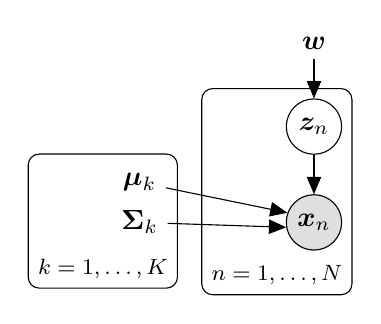
\begin{tikzpicture}
    \node[obs] (x) {$\bm{x}_n$};
    \node[latent, above=0.5cm of x] (z) {$\bm{z}_n$};
    \node[above=0.5cm of z] (pi) {$\bm{w}$};
    
    \node[left=of x, xshift=-0.5cm] (cov) {$\bm{\Sigma}_k$};
    \node[above=of cov, yshift=-1cm] (mean) {$\bm{\mu}_k$};
    
    \plate[] {plate1} {(mean)(cov)} {$k=1, \dots, K$};
    
    \plate[] {plate2} {(z)(x)} {$n=1, \dots, N$};
    
    \edge{pi}{z};
    \edge{z}{x};
    \edge{mean}{x.160};
    \edge{cov}{x.190}
    
    
    \end{tikzpicture}

\end{document}